% =====================================================================
%  DETAILED OUTLINE — REVISED MANUSCRIPT
%  "Racial Segregation and the Longevity of Black and White Americans"
%  (working title; outcome reframed from GAP to LEVELS)
%
%  This is a STRUCTURAL OUTLINE for drafting, not a finished manuscript.
%  Annotations in [[ ... ]] are notes-to-self mapping each move to the
%  revision master plan (task IDs) and the reviewer comments it answers.
%  Strip the [[ ... ]] notes before submission.
% =====================================================================

\documentclass[11pt]{article}
\usepackage[left=1in,right=1in,top=1in,bottom=1in]{geometry}
\usepackage{amsmath}
\usepackage{setspace}
\usepackage{enumitem}
\usepackage{xcolor}
\usepackage{natbib}
\usepackage{tikz}
\usetikzlibrary{arrows.meta,positioning,fit,backgrounds}

% Required by the tinytable output written to FigTab/ by the Analysis scripts.
\usepackage{tabularray}
\usepackage{float}
\usepackage{graphicx}
\usepackage{codehigh}
\usepackage[normalem]{ulem}
\UseTblrLibrary{booktabs}
\UseTblrLibrary{siunitx}
\newcommand{\tinytableTabularrayUnderline}[1]{\underline{#1}}
\newcommand{\tinytableTabularrayStrikeout}[1]{\sout{#1}}
\NewTableCommand{\tinytableDefineColor}[3]{\definecolor{#1}{#2}{#3}}

\usepackage[colorlinks=true,linkcolor=blue,citecolor=blue]{hyperref}

% Helper command to render the editorial notes distinctly while drafting.
% Comment out the second definition to hide all notes at once.
\newcommand{\note}[1]{{\color{gray}\small\textit{[[#1]]}}}
% \renewcommand{\note}[1]{} % <- uncomment to suppress all drafting notes

\title{Segregation, Political Economy, and The Longevity of Black and White Americans}
\author{Thelonious Goerz\\ \small Department of Sociology \\
Brooks School of Public Policy \\
Cornell University}
\date{Draft date: \today}

\begin{document}
\maketitle

% =====================================================================
\section{Abstract}
% =====================================================================
Racial segregation is widely understood to advantage White Americans at the expense of Black Americans through differing neighborhood environments. This view overlooks how segregation reshapes the political economy of places through public goods, taxation, and redistributive policy that implicate the well-being of all residents. This paper links 1905–1920 birth cohorts in the 1940 full-count Census to Social Security death records (N = 2.9 million) and uses multiple instruments and a sibling fixed effects design to estimate the effect of segregation on the longevity of Black and of White Americans A 10-point increase in segregation reduces \textit{both} Black and White longevity—by 0.44 and 0.29 years, respectively—with steeper harms for less-educated Whites. I show that abundant tax revenue, welfare spending, and SNAP funding explain substantial portions of these effects for both Black and White individuals, suggesting that political-economic dimensions of segregation operate beyond neighborhoods to shape Black and White outcomes in the same direction unequally, rather than through processes of White advantage.  

% =====================================================================
\section{Introduction}
% =====================================================================
\doublespacing

% =====================================================================
\section{Segregation and Black-White Inequalities}
% =====================================================================
Racial residential segregation by race is widely understood as a visible manifestation of Black-White inequalities of various forms \citep{blokland_outside_2008} and a mechanism of persistent racial stratification \citep{massey_effect_1987}. Black-White inequalities in the U.S. ranging from income to education to mortality are stark in size and troubling because they have remained durably large over time. Extensive scholarly research has documented how opportunities and risk are differentially distributed across Black and White neighborhoods, with risks disproportionately patterned such that Black residents live in worse off neighborhoods.

A long scholarly tradition on racial segregation has detailed the adverse outcomes of racial segregation for Blacks and Black-White inequalities \citep{hendi_where_2024,massey_effect_1987,frey_central_1979}. Researchers have often inferred that segregation is conversely advantageous for Whites despite comparatively limited empirical attention \citep{brown_structural_2024,quillian_does_2014}.The clearest evidence for this assertion can be seen in seminal work by Douglas S. Massey on raical segregation and violence: "racial segregation persists in the United States because whites benefit from it. In undermining the status and well-being of African-Americans a social problems, segregation simultaneously increases the incentives for whites to maintain the residential status quo" \cite[p.~1229]{massey_getting_1995}. 

Zero-sum expectations about the mechanisms generating Black-White inequalities are particularly salient for race relations and form the basis of Whites’ public opinions on race \citep{wetts_privilege_2018,bobo_attitudes_1996} and opposition to redistributive policy \citep{gilens_race_1996,mcghee_sum_2021}. Recent work has also salient for Black American's views regarding race relations as well \citep{warren_zero-sum_2025}. In practice, these beliefs inform Whites' resistance to residential and educational integration due to a belief that segregation produces White advantage\citep{crowder_spatial_2008,frey_central_1979,rich_backlash_2025,johnson_children_2019}. If segregation is beneficial to Whites, this implies that efforts to desegregate -- like those in the case of school segregation -- would close Black-White gaps by reducing White advantages and decreasing Black disadvantage \citep{johnson_children_2019,massey_getting_1995}.  

Scholarly and public understanding of segregation suggests a particular relationship with  Black-White inequalities; that of White gains from segregation at the expense of Black losses. Though hypotheses and conceptualizations vary across studies, there are strong expectations that segregation should be, on average, advantageous to Whites \citep{light_segregation_2019,quillian_does_2014,massey_getting_1995}. Despite an appearance of equivalency between inequalities and zero-sum relationships, Black-White inequalities are consistent with at least three underlying processes: (1) segregation is harmful to both groups, (2) segregation advantages Whites and disadvantages Blacks (zero-sum), (3) segregation disadvantages Blacks but does not affect Whites, yet existing papers rarely distinguish these explanations or explore the their consequences for understanding the mechanisms of inequality. These three processes are visualized in Figure 1. \footnote{It is important to note that zero-sum relationships are used in varied ways in the literature on racial stratification and segregation as short hand for White advangates and Black disadvantages \citep{mcghee_sum_2021}. This is worth noting because the original game theoretic definition states that zero-sum relationships are ones where gains of one individual are exactly proportional to the losses of the other \citep{von-neumann_theory_1944}. In this paper, I use zero-sum as a shorthand for relationships that create White advantage and simultaneously Black disadvantage.}

\begin{figure}[htbp]
\centering
\resizebox{\textwidth}{!}{%
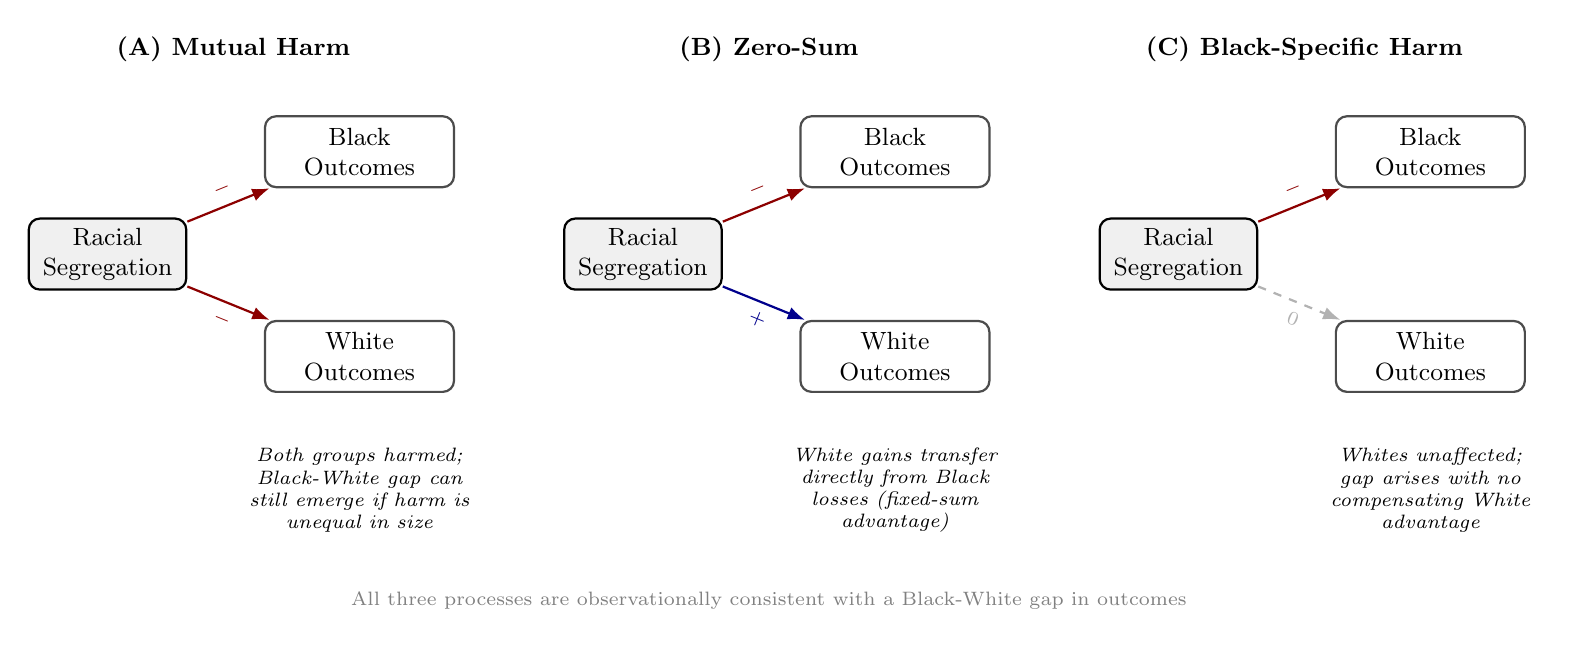
\begin{tikzpicture}[
    font=\small,
    seg/.style={draw, rounded corners, thick, fill=gray!12, align=center,
                minimum width=20mm, minimum height=9mm},
    outbox/.style={draw, rounded corners, thick, align=center,
                minimum width=24mm, minimum height=9mm},
    blk/.style={outbox, fill=white, draw=black!70},
    wht/.style={outbox, fill=white, draw=black!70},
    lbl/.style={font=\scriptsize\itshape, align=center, text width=30mm},
    panel/.style={font=\bfseries\small, align=center},
    harmarrow/.style={-{Latex[length=2.2mm]}, thick, red!55!black},
    benarrow/.style={-{Latex[length=2.2mm]}, thick, blue!55!black},
    nullarrow/.style={-{Latex[length=2.2mm]}, thick, gray!60, dashed}
]

% ---------- Panel A: Mutual harm ----------
\begin{scope}[xshift=0cm]
\node[panel] (titleA) at (1.6,2.6) {(A) Mutual Harm};
\node[seg] (segA) at (0,0) {Racial\\Segregation};
\node[blk] (blkA) at (3.2,1.3) {Black\\Outcomes};
\node[wht] (whtA) at (3.2,-1.3) {White\\Outcomes};
\draw[harmarrow] (segA) -- node[above, sloped, font=\scriptsize] {$-$} (blkA);
\draw[harmarrow] (segA) -- node[below, sloped, font=\scriptsize] {$-$} (whtA);
\node[lbl] (noteA) at (3.2,-3.0)
   {Both groups harmed;\\ Black-White gap can\\ still emerge if harm is\\ unequal in size};
\end{scope}

% ---------- Panel B: Zero-sum ----------
\begin{scope}[xshift=6.8cm]
\node[panel] (titleB) at (1.6,2.6) {(B) Zero-Sum};
\node[seg] (segB) at (0,0) {Racial\\Segregation};
\node[blk] (blkB) at (3.2,1.3) {Black\\Outcomes};
\node[wht] (whtB) at (3.2,-1.3) {White\\Outcomes};
\draw[harmarrow] (segB) -- node[above, sloped, font=\scriptsize] {$-$} (blkB);
\draw[benarrow] (segB) -- node[below, sloped, font=\scriptsize] {$+$} (whtB);
\node[lbl] (noteB) at (3.2,-3.0)
   {White gains transfer\\ directly from Black\\ losses (fixed-sum\\ advantage)};
\end{scope}

% ---------- Panel C: Black-specific harm ----------
\begin{scope}[xshift=13.6cm]
\node[panel] (titleC) at (1.6,2.6) {(C) Black-Specific Harm};
\node[seg] (segC) at (0,0) {Racial\\Segregation};
\node[blk] (blkC) at (3.2,1.3) {Black\\Outcomes};
\node[wht] (whtC) at (3.2,-1.3) {White\\Outcomes};
\draw[harmarrow] (segC) -- node[above, sloped, font=\scriptsize] {$-$} (blkC);
\draw[nullarrow] (segC) -- node[below, sloped, font=\scriptsize] {0} (whtC);
\node[lbl] (noteC) at (3.2,-3.0)
   {Whites unaffected;\\ gap arises with no\\ compensating White\\ advantage};
\end{scope}

% ---------- shared bottom caption strip ----------
\node[font=\scriptsize, gray] at (8.4,-4.4)
  {All three processes are observationally consistent with a Black-White gap in outcomes};

\end{tikzpicture}%
}
\caption{This figure describes three stylized theoretical processes consistent with an observed Black-White gap in outcomes. Solid red arrows denote a harmful ($-$) effect of segregation; solid blue arrows denote a beneficial ($+$) effect; the dashed gray arrow denotes a null effect. Only Panel (B) implies a strict zero-sum transfer of advantage from Black to White residents; Panels (A) and (C) generate the same qualitative inequality without any White benefit.}
\label{fig:zero-sum-processes}
\end{figure}

Simply identifying a gap between Black and White outcomes is ambiguous regarding the underlying relationships between mechanisms of racial stratification \citep{wrigley-field_three_2025}, the sign of the coefficients, and the resulting Black-White inequalities. From a substantive perspective, the presence of an inequality must be paired with a greater understanding of what group-specific relationships generate it to fully understand the consequences of racial stratification.

The research that directly examines the effects of segregation on White outcomes has yielded inconsistent conclusions about relationships that vary in both the direction of effects (either positive or negative) and across different outcomes  (e.g., crime, education, income). 
For instance, \citep{light_segregation_2019} find that segregation is negatively associated with White homicide victimization and positively associated with Black homicide victimization, therefore consistent with a zero-sum relationship. While \cite{quillian_does_2014} finds that segregation is negatively associated with Black educational attainment and not associated with White educational attainment.  
On the other hand, \citep{cutler_are_1997} find that segregation is negatively associated with Black educational, economic, and employment outcomes, but generally not associated or slightly negatively associated Whites' outcomes. 

These latter two studies are inconsistent with a zero-sum relationship, despite generating clear Black-White inequalities. These empirical patterns are inconsistent with zero-sum arguments but not readily accounted for by neighborhood-based theories of segregation. Though subtle, these distinction carry different takeaways about how changes to segregation relate to the widening or narrowing of inequalities. 

\section{Segregation, Neighborhoods, and Political Economy}

Much of segregation scholarship focuses on the consequences of living in racially segregated neighborhoods within segregated places. Accordingly, neighborhood effects theories and evidence are often employed to connect segregation to Black-White inequalities. As demonstrated by a voluminous literature, Black residents are more likely to live in high poverty neighborhoods \citep{massey_effect_1987,wilson_truly_1987,massey_american_1993}, be zoned for lower quality schools \citep{wodtke_are_2023,goldsmith_schools_2009}, experience higher crime exposure \citep{light_segregation_2019}, and navigate more hazardous environmental exposures \citep{wodtke_toxic_2022,elliott_historical_2013} compared to White residents. While these perspectives provide rich descriptions of how unequal distributions of various residential exposures between Black and White neighborhoods shape health and economic wellbeing, they largely overlook a burgeoning literature demonstrating that segregation shapes the political economy and of places beyond neighborhoods \citep{chyn_effects_2026,ananat_segregation_2009}.

Politics and policies have played a central role as mechanisms of racial stratification throughout history. In \textit{Black Reconstruction in America} W.E.B. DuBois highlighted how racial tensions were intentionally animated by White Southern elites for the purpose of dividing working-class Black and White workers who labored under shared working conditions. \citep[p.~700]{dubois_black_1935}. In the Jim Crow South, segregationist policies such as literacy tests and poll taxes intended to disenfranchize Black would be voters frequently excluded many poor Whites at the same time, despite racially-motivated aims \cite[p~.6]{perman_struggle_2001}.
Contemporary research on politics and racial threat point toward the conclusion that public opinion about race shapes voting patterns, which in turn have downstream consequences for the policies and politics of places \citep{gilens_race_1996,gilens_1995}. 

Whites' voting patterns are a particularly salient mechanism because segregation reduces contact between racial groups and increases the salience of racial threat \citep{blalock_1967,blumer_race_1958}. Higher racial segregation has been shown to increase the racial resentment and conservative voting patterns of non-Black voters \citep{ananat_segregation_2009}. Futhermore, \cite{chyn_effects_2026} found that racial segregation reduced support for a variety of specific policies such as support for minumum wage, redistributive spending, welfare, health spending, and opposition to police reform. These voting-related pathwways link segregation to the liberalism or conservatism of policies enacted that have implications for residents, particularly those with lower-incomes, regardless of neighborhood \citep{metzl_dying_2019}. To facilitate a concrete discussion of the different ways neighborhood and political-economic mechanisms of segregation affect outcomes,this article focuses on mortality to study the consequences of segreation. 

The striking contemporary and historical mortality disparities between Black and White populations are a particularly salient differentiation between racial groups. In 2023, the difference in life expectancy at birth between White and Black Americans was of 4.4 years \citep{arias_united_2020}. Disparities in Black and White lifespans are notable because they have remained especially persistent in light of exceptional increases in life expectancy and demographic advancements in the last 50 years. In addition to their function as health indicators, lifespan represents an important cumulative measure of life chances \citep{weber_economy_1922} and an important axis of social inequality \citep{maralani_consolidation_2021,wrigley-field_stolen_2024}. Longevity disparities have far-reaching implications for individual social networks, collective memory, culture, political participation, and social movements that would otherwise manifest if not for shortened life \citep{wrigley-field_three_2025}.

Scholarship in sociology and demogarphy has established that racial segregation is a fundamental cause of health inequality \citep{williams_racial_2001} that creates worse health outcomes for Black Americans and wide Black-White health disparities, though evidence on the health of White Americans is comparatively limited and mixed. Studies of infant health illustrate this ambiguity: \cite{austin_does_2016} found that segregation reduced the birthweight of both Black and White infants, while \cite{vu_born_2024} found negative effects on the birthweight of Black infants and no effect for White infants. Evidence on mortality is similarly inconsistent; \cite{logan_segregation_2018} found that, in certain contexts, segregation was associated with greater mortality risk for White Americans and lower risk for Black Americans, whereas \cite{karbeah_racial_2023} found that segregation increased mortality risk among both Black and White children. These divergent conclusions partly reflect methodological limitations, including reliance on death records from a single state \citep{logan_segregation_2018}. More fundamentally, existing evidence is largely correlational. Segregation covaries with features of places that are consequential for population health, thus correlational analyses cannot distinguish whether the observed relationships between segregation and mortality are causal.

\subsection{Neighborhood Effects}

According to the fundamental cause perspective, racial segregation is thought to operate through many downstream mechanisms, ranging from neighborhood exposures, socioeconomic resources, and accress to health care.\footnote{In this section, I consider both general pathways that link segregation to health as well as those particular to older adults. This is because the Data elaborated later in this study provides a snapshot of segregation observed when an individual is 65 years old.} As indicated in current literature on the social determinants of mortality and longevity, the mechanisms that shape health are often interlinked and compound over the life course \citep{breen_longevity_2024,diprete_cumulative_2006}. Rather than an exhaustive review of these machanisms, I summarize three predominant neighborhood-level mechanisms that describe the major differentiators of Black and White neighborhoods and their implications for health. 

A leading pathway linking segregation to health is through increases in poverty. Segregation increases poverty concentration \citep{massey_american_1993} and concentrates it in primarily Black neighborhoods while White neighborhoods are sheilded from it \citep{quillian_segregation_2012, ananat_wrong_2011}. Poverty has been shown to have direct implications for health through its reduction of economic resources and employment opportunities. Poverty induced by segregation could also matter for health indirectly, because poverty increases individual and environental stressors associated with worse health. Poverty is particularly consequential for the health of older adults through reductions in access to health care as well as psychosocial sress which may accelerate aging processes \citep{massey_neighborhood_2018}. Poverty may thus serve as both an direct input of worse health as well as compound existing racial inequalities in health at older ages, particularly after 60 years old \citep{geronimus_weathering_2006}.

The unequal concentration of crime and policing are also central mechanisms of segregation. Racial segregation distributes violent crime and aggressive policing spatially, concentrating both in predominantly Black neighborhoods while insulating predominantly White ones \citep{bell_anti-segregation_2020,light_segregation_2019}. This spatial concentration is consequential for health because exposure to community violence elevates depressive symptoms and psychological distress \citep{foell_exposure_2021}, and aggressive policing raises the risk of injury and death \citep{edwards_risk_2019}. Beacuse these exposures are not symmetric across groups, segregation simultaneously \textit{increases} the risk of homicide victimization for Black residents and \textit{decreases} it for White residents \citep{light_segregation_2019}. Crime and policing thus represent one of the clearest neighborhood channels through which segregation plausibly generates zero-sum outcomes. For older adults in particular, racialized exposure to crime operates beyond acute risk of victimization to create a culture of fear \citep{klinenberg_heat_2003} that shapes physiological and psychological health. The chronic stress of residing in high-violence environments contributes to accelerated physiological weathering between Black and White older adults \citep{geronimus_weathering_1992} which shapes mortality at older ages. 

Finally, racial segregation affects the quality of housing and the financial resources households can extract from them to invest in health \citep{breen_longevity_2024}. Segregation creates competition in housing markets that impose distinct costs on Black and White residents alike, though through different mechanisms. For Whites, \cite{daniels_influence_1975} documents that White renters intent on living in predominantly White neighborhoods paid a premium to segregate themselves from Black neighbors, such that the maintenance of residential separation is costly for Whites. For Black homeowners, buyers historically paid roughly a 28 percent premium to purchase homes on majority-White neighborhoods and subsequently saw those homes lose value, which eroded Black families wealth prospects \cite{akbar_racial_2025}. Because housing is the primary vehicle of wealth accumulation for most households, segregation-induced cost burdens translate into diminished resources that affect health status \citep{hurd_health_2003,wang_housing_2026}. Segregation also degrades the quality housing, particulalry for Black residents, which has important implications for health and risk of disease, particularly for older adults \citep{evans_residential_2024}. Lower-quality housing in the form of poor insulation, broken features, and lack suitable amenities are associated with poor health conditions such as the onset of disability at older ages and elevated biomarkers like c-reactive protein that proxy for environmental stressors \citep{wang_housing_2026,clair_housing_2019}. 

\subsection{Political Economy}

Each of the neighborhood pathways described operate through the composition of residential environments themselves. At least in principle, the health consequences of neighborhoods in which Black and White residents live plausibly link segregation to zero-sum outcomes. Yet, political-economic mechanisms operate at a scale beyond neighborhoods \citep{logan_political_nodate}. Taxation, spending on health and public services \citep{alesina_public_1999}, and the generosity of the safety net are shaped by voters within segregated places and set at the level of counties \citep{debenedictis-kessner_politics_2020, tausanovitch_representation_2014}. Indeed, past work has shown that segregation increases the political polarization of places, which undermines collective political efforts and in turn, spending on public services \cite{trounstine_segregation_2016}. The county-level consequences carry the scope to shape the health of all residents of a jurisdiction regardless of the neighborhood they occupy.

Recent scholarship points to the importance of considering how the increasing political polarization of places and their liberal or conservative politics and policies matter for health and wellbeing \citep{montez_us_2026,torche_political_2021}. At the county-level, important services that shape population health are delivered, such as spending on insfrastructure, health, welfare, and the level of tax revenue generated \citep{manduca_tax_2025,debenedictis-kessner_politics_2020}. Increasingly, high-levels of segregation have been linked to less-generous levels of public goods, which each have their own implications for health and wellbeing \citep{trounstine_segregation_2016,chyn_effects_2026}.

There are a variety of county-level expenditures that matter for health, but the most obvious are health and medicaid spending. Greater spending on public insurance programs have been shown to have profound effects on health and motality; for instance, \citep{goodman-bacon_public_2018} found that early medicaid adoption reduced the mortality of infants substantially and non-White child mortality by $20$ percent. Moreover, medicaid expansion was found to have particularly salient effects for older adult mortality, with \citep{miller_medicaid_2021} estimating that expansions tied to the Affordable Care Act reduced mortality by $9.4$ percent.

The level of tax revenue generated by places is critical mechanism through which places can finance policies and programs that redistribute wealth, mitigate poverty and inequality, and invest public services. Tax revenue operates as a general mechanism that can exacerbate or mitigate inequality across places that in turn affect life outcomes \citep{rauscher_variation_2022,obrien_fiscal_2025}. While health and medicaid expenditures at the county-level are directly related to health outcomes, evidence indicates that non-health spending has downstream impacts on health; \cite{mccullough_government_2016} find that higher tax revenue among other spending categories, was associated with improvements in population health and \citep{mays_evidence_2011} found that increased local public health spending reduced preventable deaths by $6.9$ percent. More generally, \citep{lobao_poverty_2012} found that greater government fiscal capacity was associated with reductions in poverty and increases in job growth which directly shape health outcomes.

In addition to taxe revenue and health expenditures nutrition and and welfare programs have direct and indirect effects on health; for instance spending on supplemental nutriction assistance (SNAP) has been shown to have direct effects on mortality; for instance, \citep{heflin_effect_2019} found that SNAP participation reduced all-cause mortality among adults ages 40--64 by $1$--$2$ percentage points. Evidence from the county-level rollout of the original Food Stamp Program points to similar conclusions over the long run, with childhood access to the program increasing adult longevity by $0.4$ percentage points \citep{bailey_is_2024} and reducing the incidence of metabolic syndrome in adulthood \citep{hoynes_long-run_2016}. Nutrition assistance thus shapes mortality both directly and through the accumulation of health over the life course.

Beyond nutrition assistance, broader welfare spending encompasses the range of transfers and services that counties provide to their poorest residents that vary considerably across counties \citep{bruch_consequences_2018}. This spending has been shown to have direct implications for mortality; for instance, \citep{fishback_births_2007} found that New Deal relief spending during the Great Depression reduced infant mortality, suicides, and deaths from infectious disease in a panel of $114$ cities. Additionally, cash transfers have been shown to have lasting consequences for longevity; for instance, \citep{aizer_long-run_2016} found that the sons of mothers accepted to the Mothers' Pension program, the first cash welfare program in the U.S.,lived approximately one year longer than the sons of rejected applicants. Contemporary evidence is more mixed, with \citep{muennig_can_2020} estimating that state supplements to the Earned Income Tax Credit improved ten-year survival among adults, while \citep{wyndham_estimating_2024} found that cash assistance had no effect on birth outcomes.

Despite a burgeoning evidence base demonstrating the importance of the political economic effects of segregation, scholarship in sociology rarely tests the extent to which these mechanisms explain the effects of segregation on the outcomes to the neighborhood-level mechanisms outlined. Determining whether the effects of segregation are more consistent with micro or macro-level mechanisms is of central importance \citep{sharkey_where_2014}. This is especially relevant in the context of recent findings tha document the rising spatial scale of segregation that reflects the separation of racial groups between places \citep{carlson_changing_2026,lichter_toward_2015}. While macro-segregation currently characterizes about half of the metropolitan areas in the U.S. in 2020 \citep{carlson_changing_2026}, the increasing overlap between racial composition and macro-level geographies demands a greater udnerstanding of how political dimensions of segregation affect individual outcomes. 

\section{The Present Study}

Thus far, the literature on segregation encompasses several mechanisms that plausibly affect mortality, though macro-level mechanisms remain at present underexplored. Neighborhood effects mechanisms broadly suggest that segregation should produce health advantages for Whites and disadvantages for Blacks, which is consistent with a zero-sum understanding of the consequences of segregation. On the other hand, political-economic mechanisms suggest broader place-level consequences that affect both Black and White residents similarly. 

The present study is organized around two empirical goals. First, I estimate the causal effect of segregation on the longevity of Black and White Americans using a set of instrumental variable strategies that induce greater geographic sorting by virtue of quasi-random spatial boundaries and a sibling fixed effects design leveraging within-family variation in neighborhood attainment. In models stratified by race, I examine how racial segregation affects Black and White longevity separately to learn about the specific relationships that underpin Black-White inequalites. This approach to analyzing mortality disparities is transparent because it provides a quantification of \textit{how} segregation affects Black and White longevity, rather than documenting observed disparities between groups. It is important to highlight that only in a scenario where the sign of the estimate on segregation is negative for Blacks and positive for Whites, would the relationship between segregation and longevity be considered zero-sum. From these analyses, I am able to recover Black-White differences in longevity from the estimates and differentiate between the underlying processes that generate inequalities.

Second, I test to the extent to which several measures of county-level spending on public goods and tax revenue explain the observed relationships between segregation and longevity. These mechanisms are (1) county tax revenue, (2) medicaid spending and health expenditures, (3) SNAP spending, and (4) welfare and cash assistance spending. While far from comprehensive, these different measures of county policy support provide a direct asessement of the level of policy liberalism with constructs and measures analagous to those used at the state-level \cite{montez_us_2020} and have storng theoretical links to individual health outcomes. This effort also builds upon the analyses in \citep{chyn_effects_2026} demonstrating that racial segregation reduces support for progressive policies by examining how much observed public spending outcomes explain the effects of segregation on health. 

% =====================================================================
\section{Data}
% =====================================================================

This study links six sources of data together to study the relationship between racial segregation and mortality: (1) individual-level data from the 1940 Census, which contains demographic information (race, gender, education, birth year); (2) linked mortality records from the CenSoc Numident data file, which contain information on year of death, place of death, and place of birth \citep{breen_censoc_2023}; (3) county-level summaries of the racial composition and segregation of places from the decennial census (1980-2000) \citep{ruggles_ipums_2023}; (4) data on historical railroad line shapefiles established before 1911 \citep{atack_historical_2016}, which are used to construct the first set of instruments; (5) county-level data on the arrangement of rivers, streams, and waterways from the TIGER/Line linear hydrography files \citep{census_tiger_2023}, which are used to construct the second set of instruments; and (6) government finance data from the Government Finance Database \citep{pierson_government_2015}, which are used to calculate county-level expenditures and tax revenues to test political-economic mechanisms.

The data cover deaths occurring between 1988 and 2005 among members of the 1905--1920 birth cohorts.
I link these sources such that each observation represents an individual and includes their demographic characteristics measured in 1940, county of birth, year and county of residence at death, and the segregation, contextual, instrument, and policy measures of the county in which they died.

\subsection{Linked 1940 Census--Numident Mortality Data}

The empirical analyses in this paper are anchored by individual-level demographic data records from the 1940 Full Count Census \citep{ruggles_ipums_2023}. To construct my analytic sample, I identify individuals from the 1905-1920 birth cohorts who were 20-35 in 1940.
These individuals are then linked to Social Security Administration (SSA) mortality records between 1988 and 2005 provided by the Berkeley CenSoc Numident file \citep{breen_censoc_2023}.
These data offer unparalleled individual-level data on mortality that are geolocated to contemporary residence at death and which are representative of the population living in the United States in 1940. The geographic specificity and rich covariates make these data ideal for analyzing spatial inequalities in mortality.
CenSoc Numident records cover deaths occurring between 1988 and 2005, allowing for reliable estimates of longevity conditional on an individual surviving to age 65 \citep{goldstein_mortality_2023}. The interpretation of longevity conditional on surviving to 65 arises because of the death window that is reliably covered by the Numident sample \citep[p.~35]{breen_censoc_2023} and is the interpretation used in \citet{breen_longevity_2024}.. The implications of this condition for the results are addressed directly in section XX>. \note{Fill in the cross-reference to the survivor-selection/double-truncation results subsection (use \textbackslash ref).}

I focus on the 1905-1920 birth cohorts for two reasons.
First, their birth years and the end year of the mortality observation window allow for plausibly complete observation of mortality that is not biased by right censorship (i.e. missing the oldest old).
In other words, those born in 1905 would be 100 years old in 2005, making it reasonable to assume that few individuals remain alive. Even for those individuals who live very long, using doubly truncated data will result in estimates biased toward zero \citep{breen_longevity_2024}, and thus produce estimates of the effect of segregation on longevity that are likely conservative.

Second, restricting to ages 20-35\footnote{\citet{halpern-manners_effects_2020} finds that the mean number of years of education of decedents in the 1940 Census is 10.4 years (1525). If we assume a normative time of starting school at 6, individuals in the sample reach the average at 16.4 years, which is well before our age cutoff.} allows for confidence that individual-level confounders to longevity, such as education status, are observed.
By conditioning on those 20 years or older, it is reasonable to assume that individuals have completed the modal level of formal education by the time that they appear in the sample.

Despite the strengths of the Numident data, there are limitations worth noting. The first is double truncation, where data are unobserved on both the left and right side of the death window (e.g., before 1988 and after 2005).
\citet{goldstein_mortality_2023} show that when not accounted for, doubly truncated mortality observation windows result in biased estimates of longevity disparities that shrink toward 0 and higher mean observed death age in samples. \footnote{The high average age at death for both Black and White individuals can be seen in Table 1 transparently and this is an artifact of truncation.}
This means that those born in 1905 are observed between the ages of 83-100 years old and those born in 1920 are observed between the ages of 68-85 years old.
Birth year fixed effects help to account for some of this bias \citep{goldstein_mortality_2023}, where individuals of varying birth cohorts may have differing numbers of years covered by the death window. However, this cannot be fully accounted for in analyses. Fortunately, a quantification of the bias is available using a Gompertz maximum likelihood technique \citep{goldstein_mortality_2023,breen_longevity_2024}, which I implement and return to in Section 8.4. 

The second limitation concerns race-specific representativeness. The CenSoc Numident file links 1940 Census data to the public release of the National Archives Record Administration ``NARA Numident'' file using the Abramitzky, Boustan, and Eriksson (ABE) exact matching algorithm \citep{abramitzky_europes_2012}. For the Numident sample, 22\% of the cases in the 1940 Census are matched to mortality records, which is concordant with other historical census matching efforts \citep[p.~7]{breen_censoc_2023}. A natural question is whether the differences in match rates are sufficient to produce bias in results when studying mortality with the Numident linked data. For Black men and women, comparisons with the 1940 Census indicate that the Numident file slightly underrepresents these groups, at $-1.8$ and $-2.4$ percent differences, respectively \citep{breen_censoc_2023}. \footnote{This matching procedure may be particularly selective for unmarried women, because of marriage-related name changes over the life course. Fortunately the Numident data contain parents' last names that can be used to link women who have undergone name change.} \citep{breen_censoc_2023} argue that bias due to representivity difference is modest when analyses are stratified by race. Nevertheless, \citet{osborne_censoc-numident_nodate} provide a set of post-stratification weights that re-weight CenSoc Numident counts to period-specific distributions of deaths to adjust for lingering selection from matching differences. To address this, I re-run models using these weights are included in appendix Table Axx.  

Additionally, analyses using sibling information, described in the Methods section, draw on a subsample of the analytic sample in which siblings can be identified within 1940 households. Siblings are identified using the ABE algorithm according to the procedure in \citep{breen_longevity_2024}, but produces a much smaller sample size than the full Numident data. The differences in individual characteristics of these samples are discussed in later sections. 


\subsection{Segregation and County Characteristics at Death}

I examine exposure to segregation in mid-to-late life, obtained and calculated based on the county individuals resided in at death.
Examining the county at death offers an empirical understanding of the effects of segregation that occurred after the Great Migration and the passage of Civil Rights Act that outlawed legal segregation.
Because much of the contemporary segregation scholarship examines the consequences of de jure segregation, this time period aligns more consistently with these theories.
Scholars recognize that the geographic scope and structure of segregation after the Great Migration are understood to be distinct from the segregation that occurred before, predominately in the South \citep{leibbrand_great_2020,grigoryeva_historical_2015}.

Despite potential limitations of using one's county at death, it is reasonable to believe that place characteristics are highly correlated with their residential experiences at birth.
\note{RA.2d / A\_RA11: reviewers called this sentence a leap of faith. State explicitly whether the birth-county fixed effects absorb \emph{historical} birth-place conditions or merely \emph{recent} sorting, and support the claim with the migration-decline-by-age evidence below.}
Patterns of neighborhood attainment and residential mobility over the life course show that the modal neighborhood transitions are to places with similar characteristics \citep{sampson_neighborhood_2008}.
Moreover, across the life-course, migration propensity declines with age \citep{bernard_life-course_2014} with individuals less likely to migrate after age 40 and, when they do, it is usually short distances \citep{molloy_internal_2011,zimran_internal_2022}.
For these reasons, segregation in the county of death likely represents a period of exposure encompassing mid-life and is correlated with earlier experiences.
However, to account for any residual variation due to early life exposures and the exceptional nature of moves during the Great Migration, I include birth county fixed effects in all models.

To measure segregation, I use the dissimilarity index (D) \citep{duncan_methodological_1955}.
The dissimilarity index measures the evenness of the distribution of Black and White residents within a county, ranging from 0-100, and is interpreted as the share of Black or White individuals that would have to move to a different neighborhood for the racial composition of neighborhoods to be the same as the racial composition of the county.
The dissimilarity index is widely used in prior work \citep{hendi_where_2024,light_segregation_2019,massey_american_2003,cutler_are_1997} because it is straightforward to calculate, concordant with past empirical evidence, and has a concrete interpretation.The dissimilarity index for the county an individual resided in at the time of their death is calculated formally in Equation (1):

\begin{equation} 
D = \frac 1 2 \sum_i^N | \frac{b_i}{B} - \frac{w_i}{W}| \times 100 
\end{equation}

Where N is the number of counties, $b_i$ and $w_i$ are the proportion of Black and White residents in the $i$th census tract and B and W are the proportion of Black and White residents in the county.
The dissimilarity scores are calculated from decennial Censuses 1980, 1990 and 2000, which correspond to the year of death observed for sample members. Although widely used and the interpretation convenient the D is well known to suffer from various index biases, outlined in \citet{fossett_new_2017} and others \citep{winship_revaluation_1977,carrington_measuring_1997}, particularly as they relate to temporal comparisons and variability in the population composition and relative group size of counties. Accordingly, in supplemental analyses, I replicate the main results with a bias-adjusted D index that adjusts for this bias \citep{fossett_new_2017}\footnote{In contrast to D, the bias-adjusted D measure is more complex to estimate and the interpretation less concrete \citep[p.~233]{fossett_new_2017}. For these reasons, I use the conventional dissimilarity index for main analyses.}. 

\note{Clarify tract coverage across decades: tracts do not cover all counties in 1980; state how untracted or partially tracted counties are handled when computing D.}

\subsection{Instrument Data: Railroads and Waterways}

I construct the instruments used in analyeses from two sources of geospatial data.
First, I use Jeremy Atack's historical GIS database of U.S. railroads, which digitizes the network of rail lines placed in operation between 1826 and 1911 \citep{atack_historical_2016}.
Retaining all segments in operation by 1911, I overlay the historical rail network on county boundaries and construct the Railroad Division Index (RDI) developed by \citet{ananat_wrong_2011}, which is described in detail in the Methods section. I also compute an indicator for any pre-1911 railroad, total track length, and track density (kilometers of track per square kilometer of land area).

Second, I measure the arrangement of rivers and streams within counties using the U.S. Census Bureau's TIGER/Line linear hydrography shapefiles \citep{census_tiger_2023}, in the spirit of the topographical instruments introduced by \citet{cutler_are_1997}. From these files, I retain natural stream and river features and exclude man-made canals, ditches, and artificial connectors, which are plausibly endogenous to development.

\subsection{Political-Economy Mechanism Data}

To measure county-level political-economic mechanisms, counties are linked to government finance records from the Government Finance Database (GFD), a compilation of Census of Governments and Annual Survey of Governments finance data \citep{pierson_government_2015}.
From the GFD, I extract the finances of county governments and construct measures of total tax revenue (including property and individual income tax components), health and hospital expenditures, Medicaid vendor payments, education spending, and direct welfare and cash assistance spending. Because government units are surveyed at varying frequencies, finance records are summed within each county-year and then averaged within the decade windows corresponding to the death decades observed in the sample (1980--1989, 1990--1999, and 2000--2005), so that each individual is assigned the policy environment of the decade in which they died.
Each measure is expressed per 1{,}000 county residents using decennial census population denominators.
\note{Dollars are currently nominal decade averages (Code/04\_policy\_data.R); decide whether to deflate to constant dollars and, if so, state the base year.}

\subsection{Analytic Sample}

My main analytic sample consists of ($N = X,XXX,XXX$) individuals residing in $X$ counties at their time of death over three decades from 1980-2000 .
The resulting counties are filtered from all counties in the U.S. such that they have a Black population greater than 0 and coverage of the RDI instrument \footnote{The data filtering procedure and stepwise sample sizes are included in table A1 in the Appendix.}.
\note{Update the filtering criteria, footnote, and Table A1 (FigTab/Filtering\_table.tex): the sample previously also conditioned on non-missing 1967 Census of Governments finance measures used for the government-fragmentation instrument, which is now removed. Restate the filtering steps for the railroad and river instruments (e.g., counties with valid RDI/hydrography measures) and report the new stepwise Ns.}

Table 1 displays the individual and county characteristics of the 1905-1920 birth cohorts, separately for Black and White decedents, across the full data, the IV sample, and the flexible sibling sample.

\begin{table}
\centering
\begin{talltblr}[         %% tabularray outer open
caption={Representativeness of Analytic Samples by Race},
note{}={Cell entries are unweighted means with standard deviations in parentheses. The IV sample is restricted to counties with non-missing railroad division index and to individuals with non-missing analytic covariates. The sibling sample is the flexible sibling-group match on the full data and is not restricted to counties with non-missing railroad division index data, so it is not a subset of the IV sample.},
]                     %% tabularray outer close
{                     %% tabularray inner open
colspec={Q[]Q[]Q[]Q[]Q[]Q[]Q[]},
colsep=4pt, row{1-Z}={font=\small},
column{3,5,7}={}{halign=c,},
column{1}={}{halign=l,},
cell{2}{2}={}{halign=c,},
cell{2}{4}={}{halign=c,},
cell{2}{6}={}{halign=c,},
cell{3}{2}={}{halign=c,},
cell{3}{4}={}{halign=c,},
cell{3}{6}={}{halign=c,},
cell{4}{2}={}{halign=c,},
cell{4}{4}={}{halign=c,},
cell{4}{6}={}{halign=c,},
cell{5}{2}={}{halign=c,},
cell{5}{4}={}{halign=c,},
cell{5}{6}={}{halign=c,},
cell{6}{2}={}{halign=c,},
cell{6}{4}={}{halign=c,},
cell{6}{6}={}{halign=c,},
cell{7}{2}={}{halign=c,},
cell{7}{4}={}{halign=c,},
cell{7}{6}={}{halign=c,},
cell{8}{2}={}{halign=c,},
cell{8}{4}={}{halign=c,},
cell{8}{6}={}{halign=c,},
cell{9}{2}={}{halign=c,},
cell{9}{4}={}{halign=c,},
cell{9}{6}={}{halign=c,},
cell{10}{2}={}{halign=c,},
cell{10}{4}={}{halign=c,},
cell{10}{6}={}{halign=c,},
cell{11}{2}={}{halign=c,},
cell{11}{4}={}{halign=c,},
cell{11}{6}={}{halign=c,},
cell{12}{2}={}{halign=c,},
cell{12}{4}={}{halign=c,},
cell{12}{6}={}{halign=c,},
cell{13}{2}={}{halign=c,},
cell{13}{4}={}{halign=c,},
cell{13}{6}={}{halign=c,},
cell{14}{2}={}{halign=c,},
cell{14}{4}={}{halign=c,},
cell{14}{6}={}{halign=c,},
cell{15}{2}={}{halign=c,},
cell{15}{4}={}{halign=c,},
cell{15}{6}={}{halign=c,},
cell{16}{2}={}{halign=c,},
cell{16}{4}={}{halign=c,},
cell{16}{6}={}{halign=c,},
cell{17}{2}={}{halign=c,},
cell{17}{4}={}{halign=c,},
cell{17}{6}={}{halign=c,},
cell{18}{2}={}{halign=c,},
cell{18}{4}={}{halign=c,},
cell{18}{6}={}{halign=c,},
cell{19}{2}={}{halign=c,},
cell{19}{4}={}{halign=c,},
cell{19}{6}={}{halign=c,},
cell{20}{2}={}{halign=c,},
cell{20}{4}={}{halign=c,},
cell{20}{6}={}{halign=c,},
cell{21}{2}={}{halign=c,},
cell{21}{4}={}{halign=c,},
cell{21}{6}={}{halign=c,},
cell{1}{2}={c=2,}{halign=c, halign=c,},
cell{1}{4}={c=2,}{halign=c, halign=c,},
cell{1}{6}={c=2,}{halign=c, halign=c,},
}                     %% tabularray inner close
\toprule
& Full Data &  & IV Sample &  & Sibling Sample &  \\ \cmidrule[lr]{2-3}\cmidrule[lr]{4-5}\cmidrule[lr]{6-7}
Variable & Black & White & Black  & White  & Black   & White   \\ \midrule %% TinyTableHeader
Age at Death                     & 81.55      & 82.05      & 81.55      & 82.05      & 80.82      & 81.53      \\
& (6.02)     & (5.66)     & (6.02)     & (5.66)     & (5.81)     & (5.48)     \\
Male                             & 0.42       & 0.44       & 0.42       & 0.44       & 0.44       & 0.47       \\
& (0.49)     & (0.50)     & (0.49)     & (0.50)     & (0.50)     & (0.50)     \\
Education (Years)                & 7.57       & 10.44      & 7.57       & 10.44      & 8.14       & 10.47      \\
& (3.50)     & (3.02)     & (3.50)     & (3.02)     & (3.48)     & (2.91)     \\
Married (In 1940)                & 0.55       & 0.49       & 0.55       & 0.49       & 0.44       & 0.39       \\
& (0.50)     & (0.50)     & (0.50)     & (0.50)     & (0.50)     & (0.49)     \\
Migrated (Birth to Death County) & 0.27       & 0.30       & 0.27       & 0.30       & 0.30       & 0.32       \\
& (0.44)     & (0.46)     & (0.44)     & (0.46)     & (0.46)     & (0.47)     \\
Reside in South at Death         & 0.61       & 0.30       & 0.61       & 0.30       & 0.59       & 0.27       \\
& (0.49)     & (0.46)     & (0.49)     & (0.46)     & (0.49)     & (0.44)     \\
County D at Death                & 0.57       & 0.53       & 0.57       & 0.53       & 0.56       & 0.52       \\
& (0.20)     & (0.17)     & (0.20)     & (0.17)     & (0.19)     & (0.17)     \\
County Population (1000s)        & 1,003.44   & 759.70     & 1,003.67   & 760.17     & 1,007.71   & 721.53     \\
& (1,777.88) & (1,469.92) & (1,778.16) & (1,470.77) & (1,811.77) & (1,406.21) \\
County Pr. Black                 & 0.26       & 0.10       & 0.26       & 0.10       & 0.25       & 0.09       \\
& (0.17)     & (0.11)     & (0.17)     & (0.11)     & (0.17)     & (0.11)     \\
N                                & 125,122    & 2,290,150  & 125,075    & 2,287,138  & 12,314     & 414,884    \\
\bottomrule
\end{talltblr}
\end{table}


\note{Model-paper move worth copying: after Table 1, add 2--3 sentences narrating the key comparisons (as Donahue \& Torrats-Espinosa do for their Tables 1 and 3), e.g., how in-sample individuals compare to out-of-sample cohort members on race, education, and region.}



% =====================================================================
\section{Empirical Strategy}
% =====================================================================
%\note{Biggest empirical upgrades live here: multilevel estimation (A\_RA8),
%the three-instrument exclusion-restriction defense (EiC.2/RI.6), sibling
%FE (A\_EiC3), and the mediation/MSEM apparatus for the mechanism test
%(B\_RA10 / B\_RE3). Keep Eq.(2) but update the estimator.}
%
%\subsection{Estimand and the level outcome}
%\begin{itemize}[leftmargin=1.5em]
%  \item Define the estimand as the effect of a 10-point change in D on \emph{the level} of longevity, estimated \emph{within} each racial %group. \note{A\_RI1 again --- make the model object match the title and theory}
%  \item Be explicit that the Black--White gap implied by the two estimates is reported as a derived contrast, with a sign interpretation tied %to H1 vs.\ H2.
%\end{itemize}
%
%\subsection{Instrumental-variables identification}
%\begin{itemize}[leftmargin=1.5em]
%  \item Restate the three IV assumptions (relevance, exclusion, monotonicity).
%  \item \textbf{First stage / relevance:} report F-stats for all three instruments. \note{keep the strong-first-stage evidence}
%  \end{itemize}
%  

Despite the relative strengths and limitations of each strategy the IV and sibling fixed effects approaches are strengthened when paired together. These designs rely on different assumptions for identifying causal effects and and different limitations. Because, for example, sibling designs do not require the same exclusion restriction assumptions as the instruments, then consistent estimates across designs suggest that exclusion violations do not drive results, which allows for the triangulation of a plausibly causal effect. 

Instrumental variable designs are powerful because they offer a high degree of geographic representation in the sample, but rely on strong assumptions regarding exclusion that are difficult to test in many empirical settings. To address these limitations, I utilize several different complementary instruments and an alternative sibling fixed effects design to triangulate the effects of segregation on longevity. I describe each of these approaches in detail. 

The first strategy uses a set of instruments that rely on a logic of spatial fragmentation with that result from different sources; these sources are government density, natural river and topological divisions, and historic railroad patterns established well before the period of observation. The core logic that underpins the instrument strategy is the proposition that a greater spatial division of a county facilitates more natural spatial segregation to take place. I adapt two instruments employed in the literature to the county setting that plausibly induce greater segregation. Each of these instruments relies on the same logic, but with varying degrees of credibility regarding their potential exclusion restriction violations. 

The preferred instrumental variable strategy is the railroad division index (RDI) proposed by \citep{ananat_wrong_2011}. This instrument is constructed for counties using historical railroad shapefiles sourced from \citep{atack_new_1994} (check cite). The RDI measures the extent to which counties are divided up by intersections historical railroad lines that were established in the early 20th century. The railroad division index calculates the number of intersections that a county has with rail lines in a standardized index that ranges from 0 to 1, with higher values indicating more division. In addition to rail lines, I also instrument with the density of railroad tracks per square kilometer of the county. The RDI equation is described as follows: 

defined as $RDI = 1 - \sum_i (a_i/A)^2$, where $a_i$ is the area of each subpolygon created by cutting the county with the rail network and $A$ is the total county area. The index equals 0 for counties left undivided by railroads and approaches 1 as rail lines subdivide a county into many small pieces, capturing the physical partitioning of places that facilitated racially divided neighborhood boundaries.

The intuition behind the RDI is that historical railroads provided natural barriers within places that populations could cluster around, thus creating higher levels of baseline segregation. \citep{ananat_wrong_2011} also demonstrates that historical accounts of White segregationist efforts often utilized natural barriers such as rail lines to establish communities and neighborhoods, because these barriers are naturally difficult to navigate. There are two leading issues that may undermine exclusion. First in the original \citep{ananat_wrong_2011} paper, the RDI is constructed for Northern metropolitan areas,  because the majority of African Americans lived almost entirely in the South before the 1900s when the railroads were laid. Therefore only in non-Southern cities can railroad configuration be treated as exogenous to race and thought to induce segregation by Black inflows from the great migration. This poses challenges for the county-level geography available in the Census as well limits the geographic generalizability of these estimates. I examine the consistency of results using the RDI in models stratified by those living in the South versus the non-South (appendix table Axx). 

Second, it is important to note that while railroad division does not directly relate to railroad \textit{exposure} per se, they are inherently related. The exclusion restriction hinges on the assumption that early 20th Century railroads do not affect mortality directly. On one hand, railroads could affect mortality by generating financial prosperity in areas surrounding tracks which could promote better health. \citep{black_impact_2015}, using railroad proximity to instrument for migration, they show that railroads had little association with economic outcomes for a non-selective group of Southern-born White older adults, indicating that the long-term health impacts of railroad induced prosperity are likely minimal. To test this possibility directly, I regress education and income of 1905-1920 birth cohorts in 1940 on the RDI to test whether railroad division is directly related to socioeconomic outcomes. I conduct this procedure for those that did not migrate during their lifetime to capture the potential impact of the RDI for those exposed continuously to the same place as well as the full sample to capture the relationship between exposure to the RDI in one's county at death (appendix tables Axx). These tests indicate that the RDI is not significantly associated with the educational attainment of Blacks or Whites, regardless of sample. However, the RDI is associated actually slightly negatively associated income for Blacks and Whites at a similar magnitude ($-.04$). However it is important to note the small magnitude of this association. The RDI ranges from 0-1, indicating that a one point increase in railroad division (RDI/100) would translate to approximately a $0.004\%$ decrease in earnings in 1940. While these estimates are significantly negative, they are quite insignificant substantively. \footnote{It is important to highlight that the regression results for income and education for those who did not migrate during their lifetime (i.e., those that were can confidently attribute their RDI value to birth place as well as death place) are highly similar to the full sample results, suggesting that whether we capture RDI exposure early or later in life, any impacts do not appear to compound over time in ways that exacerbate exclusion restriction violations.}

On the other hand, railroads could also result in increased hazards such as pollution and or negative environmental externalities that harm health \citep{dockery_association_1993}. In particular, small particulate matter in the air has resulting from exhaust and emissions is associated with poor health outcomes \textbf{[cites]}. To test the extent to which the RDI could directly affect health through pollution, I examine the relationship between the RDI and small Particulate Matter (PM2.5) concentration $PM2.5/m^3$ and railroad division in U.S. counties in 1999 and 2000. \footnote{Prior to the 1990s, the Environmental Protection Agency did not collect data on PM2.5 levels. Modeled estimates are available for earlier periods, but may be subject to bias.}. PM2.5 measures the concentration of tiny dust and soot particles in the air in micrograms per cubic meter ($\mu /m^3$), with an safe range concentration ranging between 0-9 within an area. Tests of the association between RDI and PM2.5 concentration are positively and significantly associated, but the magnitude is very small. Going from a county that has no railroad division to one that is completely divided by rail lines represents a difference in PM2.5 concentration of $.356$ that, while significantly associated, is quite small in magnitude (appendix Axx). 

Despite evidence presented against exclusion violations owing to direct effects of the RDI on health, it is nevertheless possible that the RDI could operate through other pathways. I further address these potential violations by complementing these IV estimates using an additional instrument set and a sibling fixed effects identification strategy. 

The second set of instruments employed are the the density of rivers and streams within a county \footnote{It is important to note that each of these instruments spatial division instruments will be correlated to some degree, as demonstrated in the appendix figure (Axx), however the correlation between instruments is relatively weak. Across all pairwise correlations the instruments range from an $R^2$ value of $x$ to $xx$. These relatively low values indicate that each of these instruments is picking up on a different dimension of spatial division in an area rather than substituting for another measure. }. The logic of using natural streams and rivers to instrument for segregation relies on the quasi-randomness of natural boundaries. Instruments of the form of rivers and streams have been employed in several studies on the consequences of segregation \citep{trounstine_segregation_2016,cutler_are_1997} that naturally induce places to be more or less segregated. While railroads and highways have been used historically to segregate, these natural boundaries are arguably less subject to these sources of bias because they are far more difficult for humans to manipulate for other aims and they do not correspond to other administrative functions that may induce a spurious relationship between the instrument and mortality. 

For each county, I compute the number of distinct named rivers and its square, following the quadratic specification in \citet{cutler_are_1997}, along with the count of stream features, total stream length, and stream density.

Thus far, different instrument strategies carry the shared concern that there could be some sort of exclusion restriction violations posed due to their physical and geographic nature that could be affect health. To complement these estimation approaches, I utilize a sibling fixed effects identification strategy. The sibling fixed effects strategy is advantageous because it relies on different assumptions and sources of identifying variation to establish a causal relationship between segregation and longevity. Sibling fixed effects adjust for all characteristics common to individual and family background characteristics of siblings by differencing out common features. After controlling for individual demographic characteristics that vary across siblings, we identify the effect of segregation on longevity from differences in siblings residential environments. While sibling fixed effects require more modest assumptions, but may be limited by external validity concerns, because they rely on a sample subset of matched sibling pairs and much smaller sample sizes. 
%\begin{itemize}
%  \item \textbf{Monotonicity:} keep the decade-over-decade $R^2$ decline evidence.
%  \item Interpret estimates as a LATE; note the over-identification-test caveat (large-$N$ rejection is uninformative). \note{keep existing %footnote logic}
%\end{itemize}
%
%\subsection{Sibling fixed effects (family-level selection)}
%\note{A\_EiC3 / EiC.3 --- residential selection. Sibling FE handles
%family-of-origin selection into places. State clearly that it addresses
%\emph{family-level} selection, not all selection, and that it converges
%with the IV (this convergence is the GO/NO-GO pass).}
%
%\subsection{Mechanism / mediation models}
%\note{B\_RE3 / B\_RA10 / C\_RA6 --- the new explanatory contribution. This
%subsection didn't exist before.}
%\begin{itemize}[leftmargin=1.5em]
%  \item Specify the mediators: taxes, Medicaid, welfare, SNAP, Montez policy-liberalism index.
%  \item Explain logic of mechanism testing -- e.g., we are trying to capture macro -- not estimate the quantitiy that is due to neighborhood %effects. For the data that we have, we are only able to see individuals' county of residence, rather than their neighborhood. Future work %should test this. 
%  \item State what ``partial mediation'' will and won't license as a claim. \note{C\_RI3 / RI.3 --- the evidence supports a \emph{mediated} %(policy) account over a \emph{direct}-exposure claim; say so}
%\end{itemize}
%
%\subsection{Robustness and weight-of-evidence}
%\begin{itemize}[leftmargin=1.5em]
%  \item Post-stratification weights; alternative segregation indices (Theil H, isolation, bias-adjusted D).
%  \item Cohort-bin and education-heterogeneity checks. \note{B\_EiC7 / EiC.7 --- assemble these into an explicit weight-of-evidence subsection}
%  \item year bin to check the robustness to plausible military service 
%  \item 
%  \item \textbf{Older-age migration check.} \note{RE.6 / B\_RE6 --- ``returning home to die,'' retirement moves; test sensitivity to late-life %migration}
%\end{itemize}

% =====================================================================
\section{Results}
% =====================================================================
\note{Reorder so the level results for each group come first and the gap is
read off them; then heterogeneity; then mechanism. Fold magnitude
comparisons in here (RI.8).}

\subsection{Descriptives}

\subsection{Main effect on longevity levels, by race}
\begin{itemize}[leftmargin=1.5em]
  \item OLS/multilevel associations first (both groups negative).
  \item \textbf{IV estimates --- the headline.} A 10-point rise in D lowers \emph{both} Black and White longevity levels; report updated multilevel point estimates and CIs. \note{report whatever the re-estimated numbers are; the OLD numbers were 0.44 / 0.29 --- update}
  \item \textbf{Read the gap off the levels.} Black harm $>$ White harm in magnitude, but \emph{both negative} $\Rightarrow$ H2 over H1. \note{this is the level-to-gap inference you described}
  \item \textbf{Triangulation panel:} show government-fragmentation, rivers, railroad/RDI, and sibling-FE estimates side by side; they converge. \note{A\_EiC6 --- the single most persuasive figure; make it prominent}
  \item Magnitude comparisons (homeownership $\approx$4 mo; 1 yr education $\approx$4.2 mo; decline-in-segregation scenario). \note{RI.8 --- move here from discussion}
\end{itemize}

\subsection{Heterogeneity by education and gender}
\begin{itemize}[leftmargin=1.5em]
  \item Whites: harm declines with education but never vanishes (college+ still harmed). \note{supports H3}
  \item Blacks: harm roughly education-invariant. \note{supports H3 + differential-returns lit}
  \item Tie explicitly back to the DuBois-derived H3, not just reported as a subgroup split. \note{closes the loop RA flagged on front/back-end connection}
\end{itemize}


\note{Keep Gender but compress --- it's secondary.}

\subsection{Mechanism: political-economy mediation}
\note{NEW headline subsection --- B\_RE3 payoff.}
\begin{itemize}[leftmargin=1.5em]
  \item Show segregation $\rightarrow$ policy mediators $\rightarrow$ longevity.
  \item Report the mediated share of the total effect.
  \item Interpret: supports the macro/shared channel (H2) as a real pathway, not just a residual. \note{C\_RI3 --- mediated account, stated carefully}
\end{itemize}


\subsection{Double truncation and survivor selection}
\note{RE.1 / B\_RE1 --- this got one line before; expand into its own
subsection and ENGAGE the mortality-crossover literature, which reviewers
specifically named.}
\begin{itemize}[leftmargin=1.5em]
  \item Explain double truncation and birth-year FE as the standard correction.
  \item \textbf{Report the Gompertz double-truncation check} that tracks the FE estimates. \note{B\_RE1 PARTIAL --- the analysis exists; write it up}
  \item \textbf{Engage the Black--White mortality crossover} explicitly and say what it does/doesn't do to a level interpretation at 65+. \note{still-needed half of RE.1}
  \item Scope the outcome honestly as \emph{longevity conditional on survival to 65}. \note{C\_RE2 / RE.2 --- life-course nuance about what segregation ``means'' at 65+}
\end{itemize}

\subsection{Millitary and cohort variation}

% =====================================================================
\section{Discussion}
% =====================================================================
\begin{enumerate}[leftmargin=1.5em]
  \item \textbf{Restate the verdict in level terms.} Segregation lowers longevity for both groups; the zero-sum (H1) sign pattern is rejected. \note{the whole reframe lands here}
  \item \textbf{Why both groups lose: the macro channel.} The mediation results show the political-economy pathway is doing real work --- this is what neighborhood-only accounts miss. \note{C\_RA3 / the non-zero-sum case, now empirically backed}
  \item \textbf{Class gradient among Whites.} Connect to wages-of-Whiteness: the White ``benefit'' is symbolic, the harm material; least-buffered (low-ed) Whites lose most. \note{C\_RI4 payoff}
  \item \textbf{Relation to prior work} (Logan--Parman, Karbeah--Hacker, Hendi), now characterized accurately and in level terms. \note{C\_RA4}
  \item \textbf{Limitations} (tighten, honest): survival-to-65 selection + crossover; historical cohorts vs.\ contemporary attenuation; LATE/exclusion caveats; mediation is partial, not exhaustive. \note{RE.1, RE.2; exclusion caveats}
  \item \textbf{Implications.} Desegregation could raise longevity for both groups and is not a White-cost policy. Future work: contemporary cohorts, allostatic load, direct mechanism studies.
\end{enumerate}

% =====================================================================
\section{Conclusion}
% =====================================================================
\note{Short. One paragraph. The takeaway: racial stratification harms
Black AND White Americans; the zero-sum belief is a symbolic mechanism,
not a description of material reality; the harm partly flows through the
political economy of segregated places.}

% =====================================================================
\section*{Tables \& Figures (planned)}
% =====================================================================

 % Prompt: I want you to read through the text and update this list of tables wnd figures with the tables and figures that I  % reference in the text (e.g., Axx or verbally as being necessary.
\note{Reuse most existing exhibits; new/changed ones marked NEW/CHANGED.}
\begin{enumerate}[leftmargin=1.5em]
  \item Fig 1 --- Zero-sum processes
  \item Fig 2 --- OLS/multilevel level estimates by race 
  \item Fig 3 --- IV level estimates by race. \note{CHANGED --- level framing}
  \item Fig 4 --- \textbf{Triangulation panel:} all instruments + sibling FE. \note{NEW --- lead figure}
  \item Fig 5 --- IV by education, Whites. (keep)
  \item Fig 6 --- IV by education, Blacks. (keep)
  \item Fig 7 --- \textbf{Mediation: segregation $\rightarrow$ policy $\rightarrow$ longevity.} \note{NEW}
  \item Table 1 --- Representativeness (+ race-specific match quality). \note{CHANGED}
  \item Table 2 --- Descriptives by race. (keep)
  \item Table 3 --- OLS/multilevel results. \note{CHANGED}
  \item Table 4 --- IV results (level, by race). \note{CHANGED}
  \item Table 5 --- IV by gender. (keep)
  \item Table 6 --- IV by education. (keep)
  \item Table 7 --- \textbf{Mediation / MSEM results.} \note{NEW}
\end{enumerate}

\section{Appendix}
\subsection{A}
\begin{enumerate}
  \item Table 1 ---- filtering table; 
  \item Table 2 ---- F-stats
  \item Table 3 ---- 
  \item Table  ----  weighted models
  \item Table  ---- alt-index models; 
  \item Table  ---- migration check; 
  \item Table  ---- map 
\end{enumerate}

\subsection{B: Robustness checks}
\note{Compress the robustness prose into a paragraph + appendix pointer:
weights, alt indices, migration, cohort bins all concordant.}
% =====================================================================
% References
% =====================================================================
\bibliographystyle{apalike}
\bibliography{ref}

\end{document}